\documentclass[../main.tex]{subfiles}
\graphicspath{{\subfix{../images/}}}
\begin{document}

% \subsubsection{Camera–LiDAR Calibration} \label{sec:camera-lidar_results}

During extrinsic calibration, the same checkerboard images were concurrently scanned by the LiDAR.  
Each frame was held stationary while the LiDAR accumulated data over 0.5 seconds, producing a dense point cloud of the target even at ranges up to 12~m.  
These data were segmented into \acp{ROI}, matched to their corresponding image frames, and processed within MATLAB’s LiDAR Calibration tool \cite{matlab_calibration} to derive the initial extrinsic transformation.

% \begin{figure}[htbp]
%     \centering
%     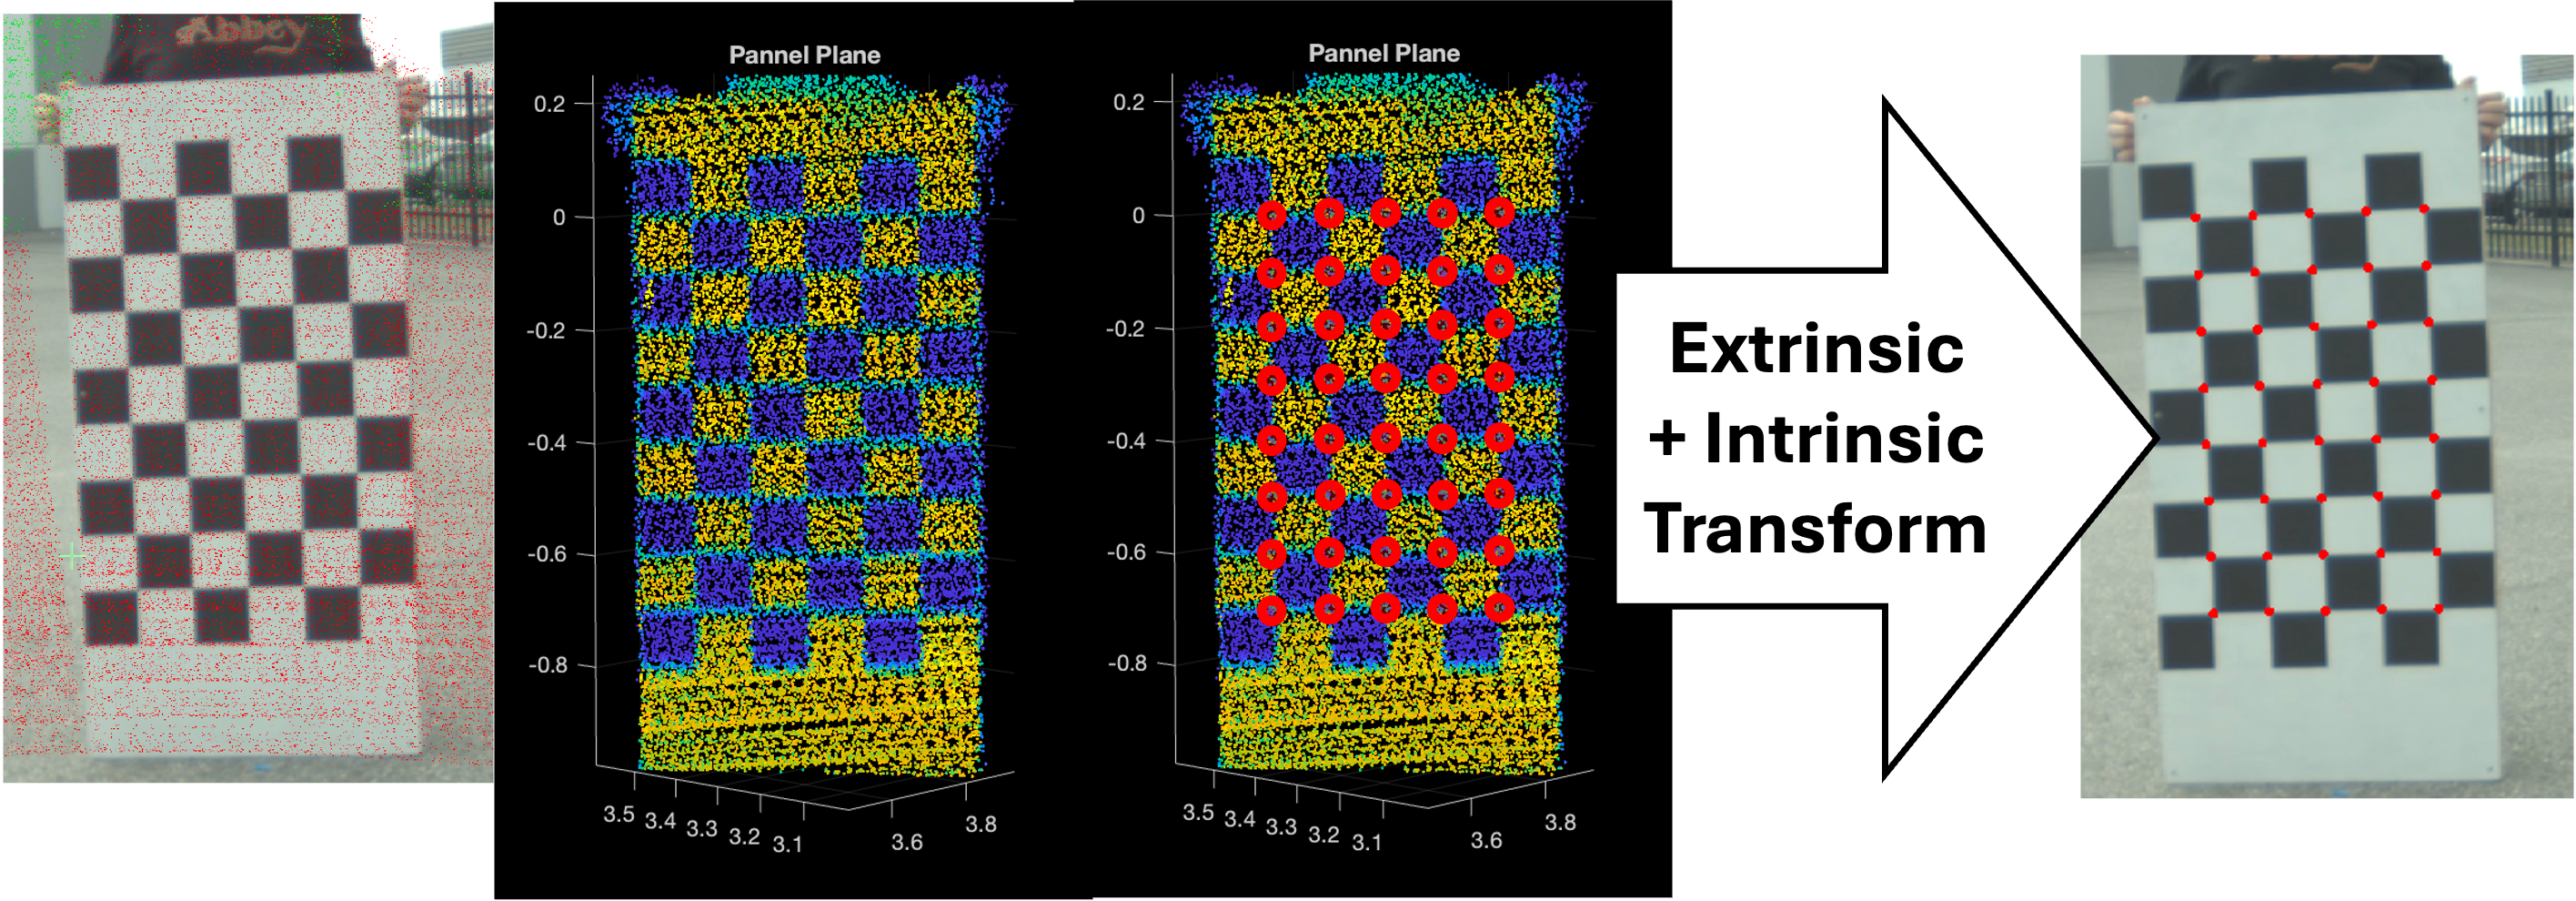
\includegraphics[width=0.8\linewidth]{Images/calib_checkers.png}
%     \caption{Example of matched LiDAR point cloud and camera checkerboard detections used for extrinsic calibration.}
%     \label{fig:calib_check}
% \end{figure}

Subsequent manual refinement was conducted by aligning environmental features visible in both modalities, such as fences, walls, and trees, as shown in Figure~\ref{fig:LiDAR_overlay3A}.  
This process improved both extrinsic and intrinsic parameter consistency and yielded substantially higher projection fidelity.  
Comparison between early and final calibration results can be seen by comparing Figures~\ref{fig:LiDAR_overlay4} and~\ref{HDR_calib_final}.

% \begin{figure}[htp]
% \begin{subfigure}{\textwidth}
% \centering
% 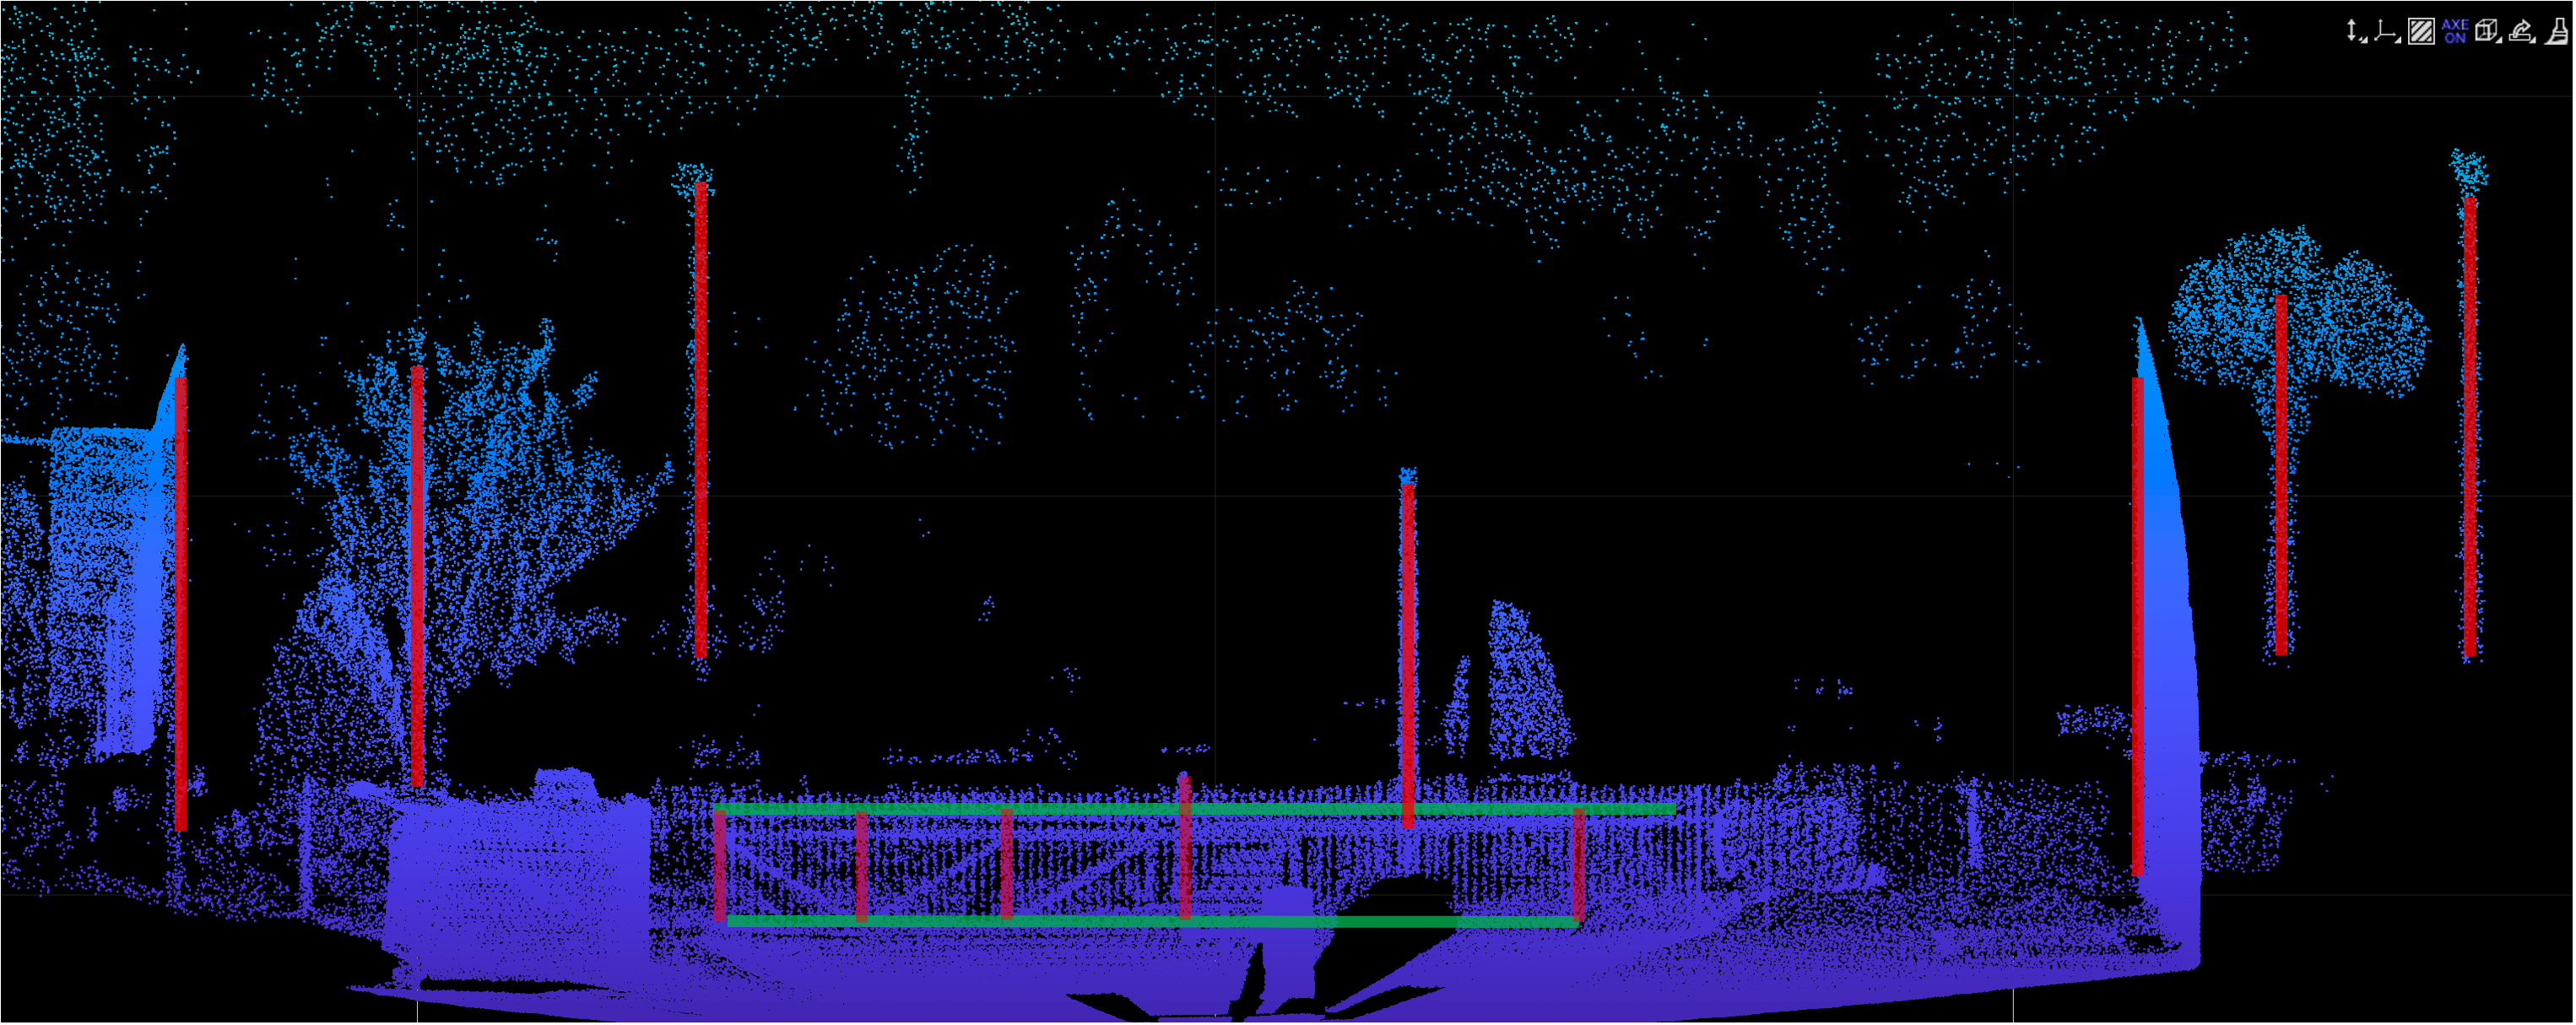
\includegraphics[width=0.94\linewidth]{Images/LiDAR_features.png}
%     \caption{}
% \end{subfigure}
% \bigskip
% \begin{subfigure}{\textwidth}
% \centering
% 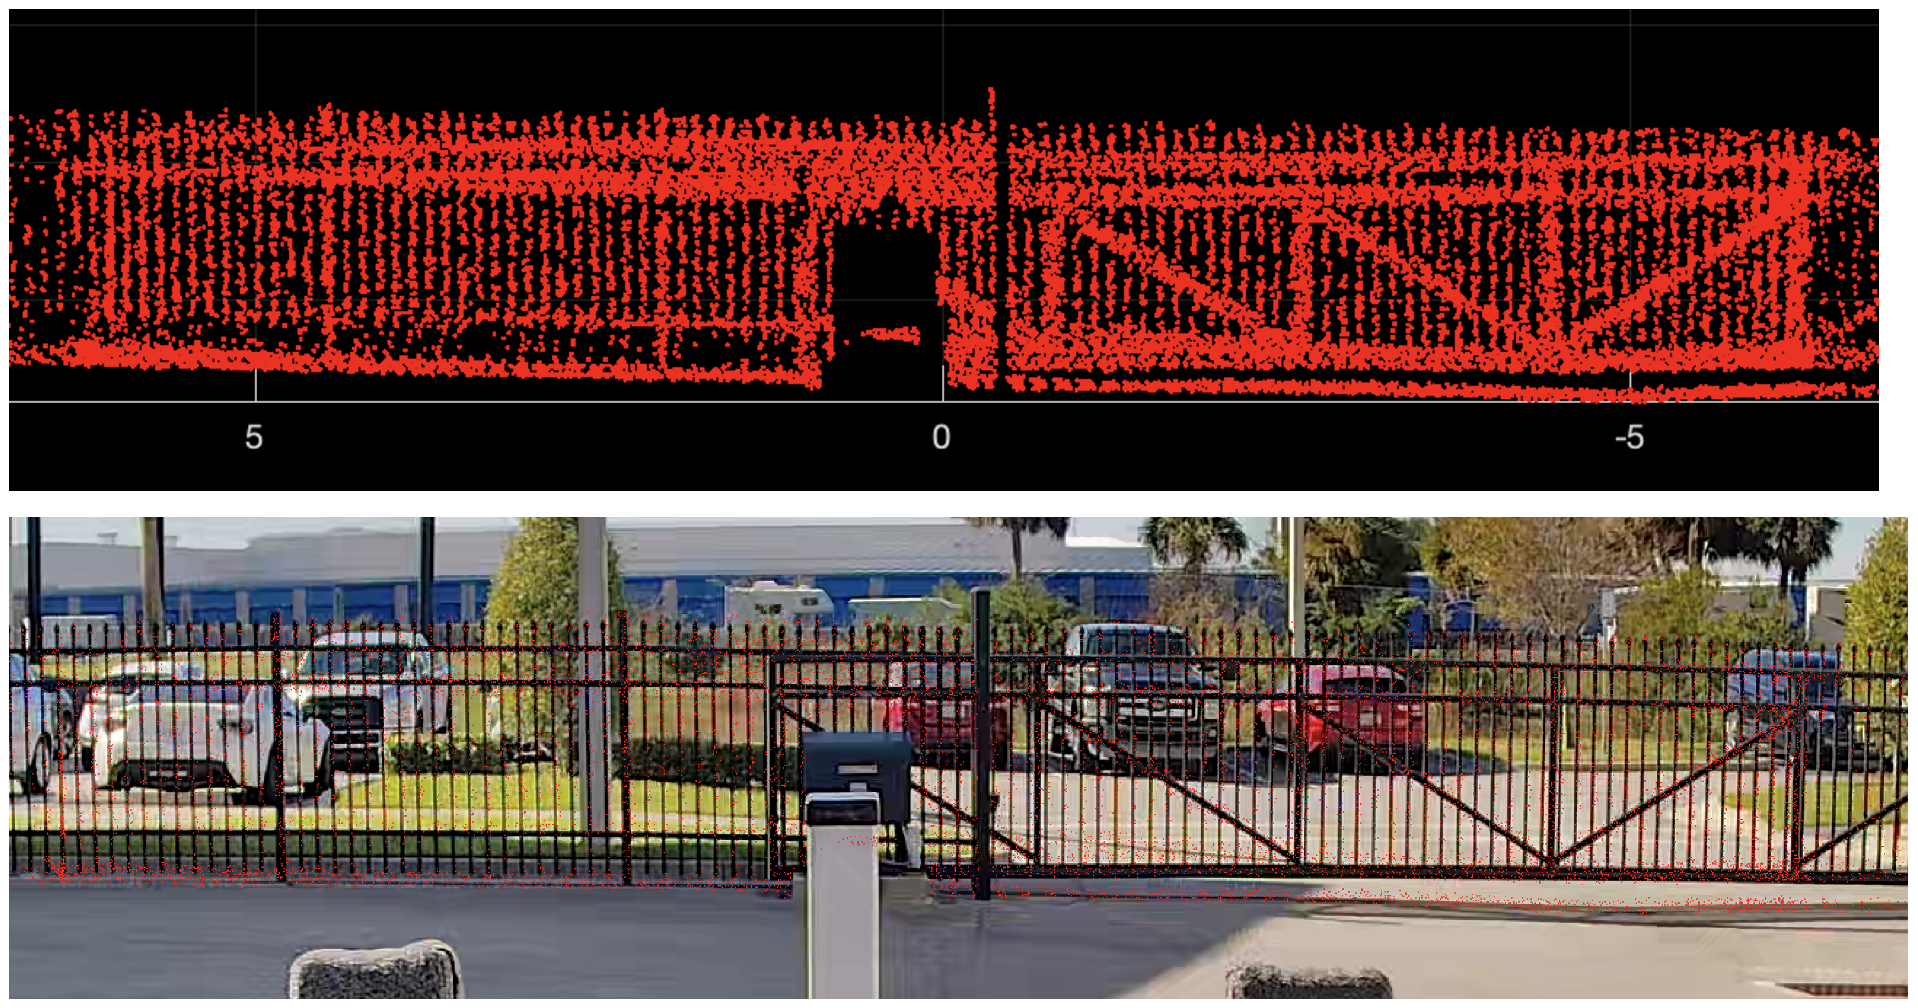
\includegraphics[width=0.94\linewidth]{Images/LiDAR_calib_fence.png}
%     \caption{}
% \end{subfigure}
% \caption{Vertical (red) and horizontal (green) macro-level features within the point cloud (a) are isolated (b) to support visual refinement of the camera–LiDAR alignment.}
% \end{figure}

% \begin{figure}[ht]
%     \centering
%     \includegraphics[width=0.8\linewidth]{Images/LiDAR_overlay4.png}
%     \caption{Initial calibration result showing early ROI-based alignment with overlaid geometric guides for evaluation.}
%     \label{fig:LiDAR_overlay4}
% \end{figure}
% \begin{figure}[htp]
% \begin{subfigure}{\textwidth}
% \centering
% \includegraphics[width=0.94\linewidth]{Images/LiDAR_overlay3A.png}
%     \caption{Three isolated regions of interest (ROI) in the LiDAR point cloud.}
%     \label{fig:LiDAR_overlay3A}
% \end{subfigure}
% \bigskip
% \begin{subfigure}{\textwidth}
% \centering
% \includegraphics[width=0.94\linewidth]{Images/LiDAR_overlay3B.png}
%     \caption{}
%     \label{fig:LiDAR_overlay3B.png}
% \end{subfigure}
% \caption{Final camera–LiDAR calibration. LiDAR ROIs containing identifiable geometry (a) are projected as red pixels onto the HDR image (b) to confirm alignment quality.}
% \label{HDR_calib_final}
% \end{figure}


\end{document}